\documentclass[aspectratio=169]{../latex_main/tntbeamer}  % you can pass all options of the beamer class, e.g., 'handout' or 'aspectratio=43'
\usepackage{dsfont}
\usepackage{bm}
\usepackage[english]{babel}
\usepackage[T1]{fontenc}
%\usepackage[utf8]{inputenc}
\usepackage{graphicx}
\graphicspath{ {./figures/} }
\usepackage{algorithm}
\usepackage[ruled,vlined,algo2e,linesnumbered]{algorithm2e}
\usepackage{hyperref}
\usepackage{booktabs}
\usepackage{mathtools}

\usepackage{amsmath,amssymb}

\DeclareMathOperator*{\argmax}{arg\,max}
\DeclareMathOperator*{\argmin}{arg\,min}

\usepackage{amsbsy}
\newcommand{\vect}[1]{\bm{#1}}
%\newcommand{\vect}[1]{\boldsymbol{#1}}

\usepackage{pgfplots}
\pgfplotsset{compat=1.16}
\usepackage{tikz}
\usetikzlibrary{trees} 
\usetikzlibrary{shapes.geometric}
\usetikzlibrary{positioning,shapes,shadows,arrows,calc,mindmap}
\usetikzlibrary{positioning,fadings,through}
\usetikzlibrary{decorations.pathreplacing}
\usetikzlibrary{intersections}
\pgfdeclarelayer{background}
\pgfdeclarelayer{foreground}
\pgfsetlayers{background,main,foreground}
\tikzstyle{activity}=[rectangle, draw=black, rounded corners, text centered, text width=8em]
\tikzstyle{data}=[rectangle, draw=black, text centered, text width=8em]
\tikzstyle{myarrow}=[->, thick, draw=black]

% Define the layers to draw the diagram
\pgfdeclarelayer{background}
\pgfdeclarelayer{foreground}
\pgfsetlayers{background,main,foreground}

% Requires XeLaTeX or LuaLaTeX
%\usepackage{unicode-math}

\usepackage{fontspec}
%\setsansfont{Arial}
\setsansfont{RotisSansSerifStd}[ 
Path=../latex_main/fonts/,
Extension = .otf,
UprightFont = *-Regular,  % or *-Light
BoldFont = *-ExtraBold,  % or *-Bold
ItalicFont = *-Italic
]
\setmonofont{Cascadia Mono}[
Scale=0.8
]

% scale factor adapted; mathrm font added (Benjamin Spitschan @TNT, 2021-06-01)
%\setmathfont[Scale=1.05]{Libertinus Math}
%\setmathrm[Scale=1.05]{Libertinus Math}

% other available math fonts are (not exhaustive)
% Latin Modern Math
% XITS Math
% Libertinus Math
% Asana Math
% Fira Math
% TeX Gyre Pagella Math
% TeX Gyre Bonum Math
% TeX Gyre Schola Math
% TeX Gyre Termes Math

% Literature References
\newcommand{\lit}[2]{\href{#2}{\footnotesize\color{black!60}[#1]}}

%%% Beamer Customization
%----------------------------------------------------------------------
% (Don't) Show sections in frame header. Options: 'sections', 'sections light', empty
\setbeamertemplate{headline}{empty}

% Add header logo for normal frames
\setheaderimage{
	% 
\includegraphics[height=\logoheight]{figures/TNT_darkv4.pdf}
	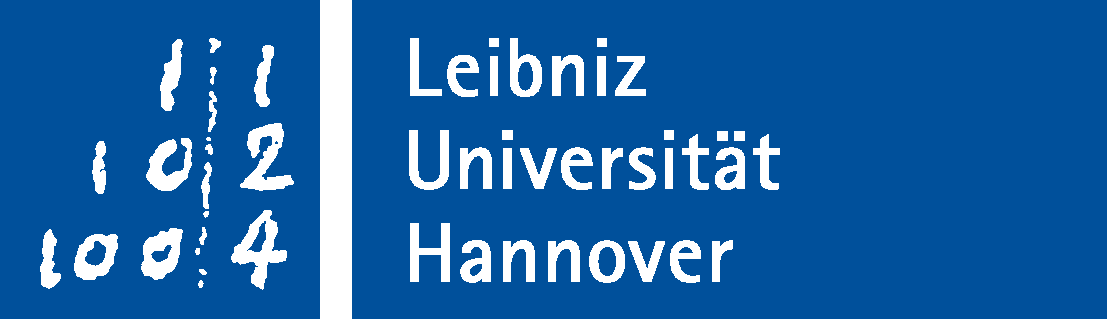
\includegraphics[height=\logoheight]{../latex_main/figures/luh_logo_rgb_0_80_155.pdf}
	% 
\includegraphics[height=\logoheight]{figures/logo_tntluh.pdf}
}

% Header logo for title page
\settitleheaderimage{
	% 
\includegraphics[height=\logoheight]{figures/TNT_darkv4.pdf}
	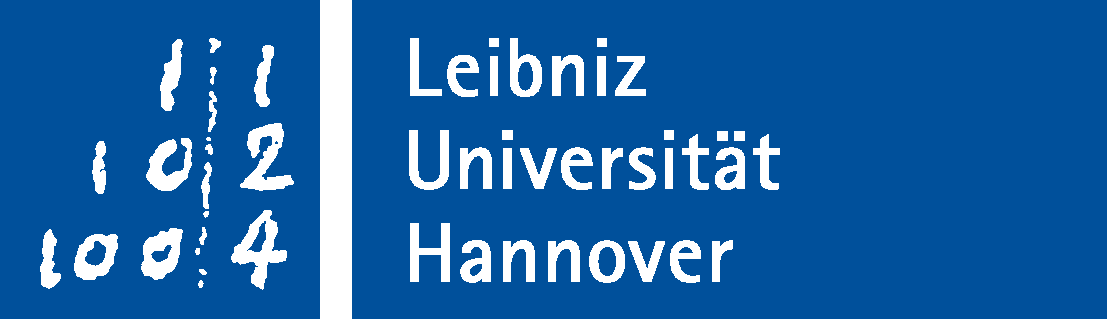
\includegraphics[height=\logoheight]{../latex_main/figures/luh_logo_rgb_0_80_155.pdf}
	% 
\includegraphics[height=\logoheight]{figures/logo_tntluh.pdf}
}

% Title page: tntdefault 
\setbeamertemplate{title page}[tntdefault]  % or luhstyle
% Add optional title image here
%\addtitlepageimagedefault{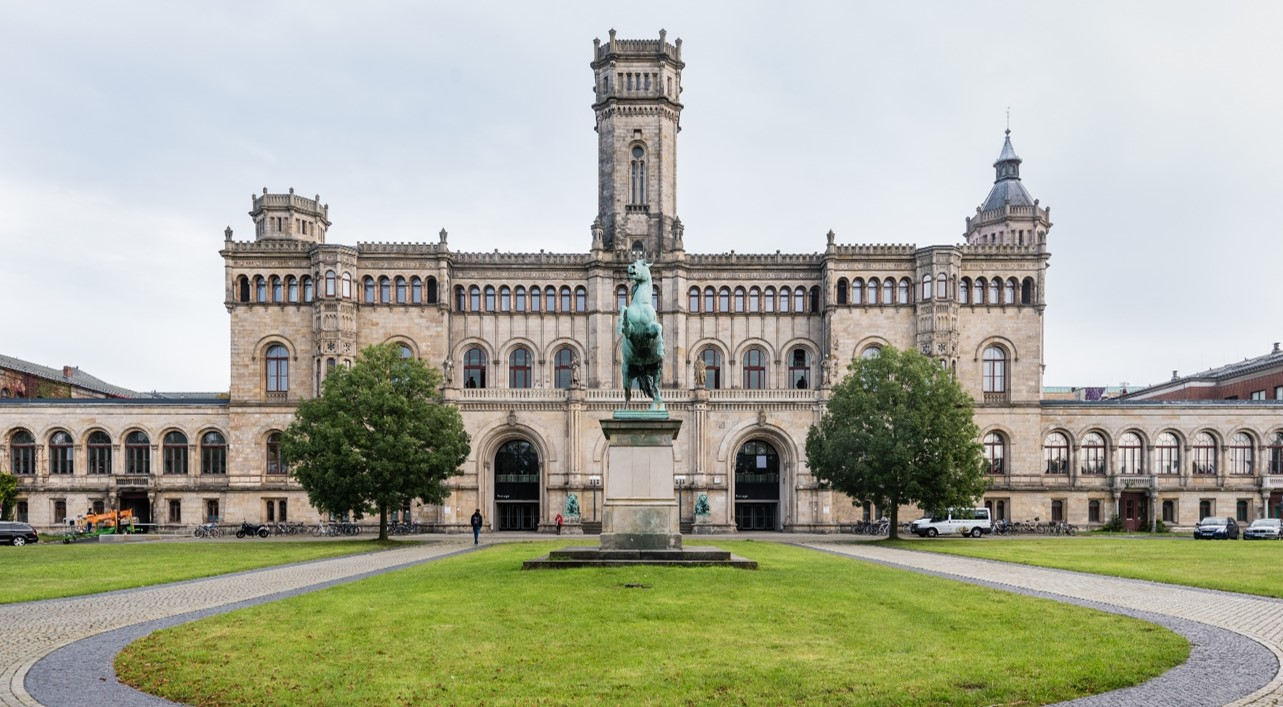
\includegraphics[width=0.65\textwidth]{figures/luh_default_presentation_title_image.jpg}}

% Title page: luhstyle
% \setbeamertemplate{title page}[luhstyle]
% % Add optional title image here
% \addtitlepageimage{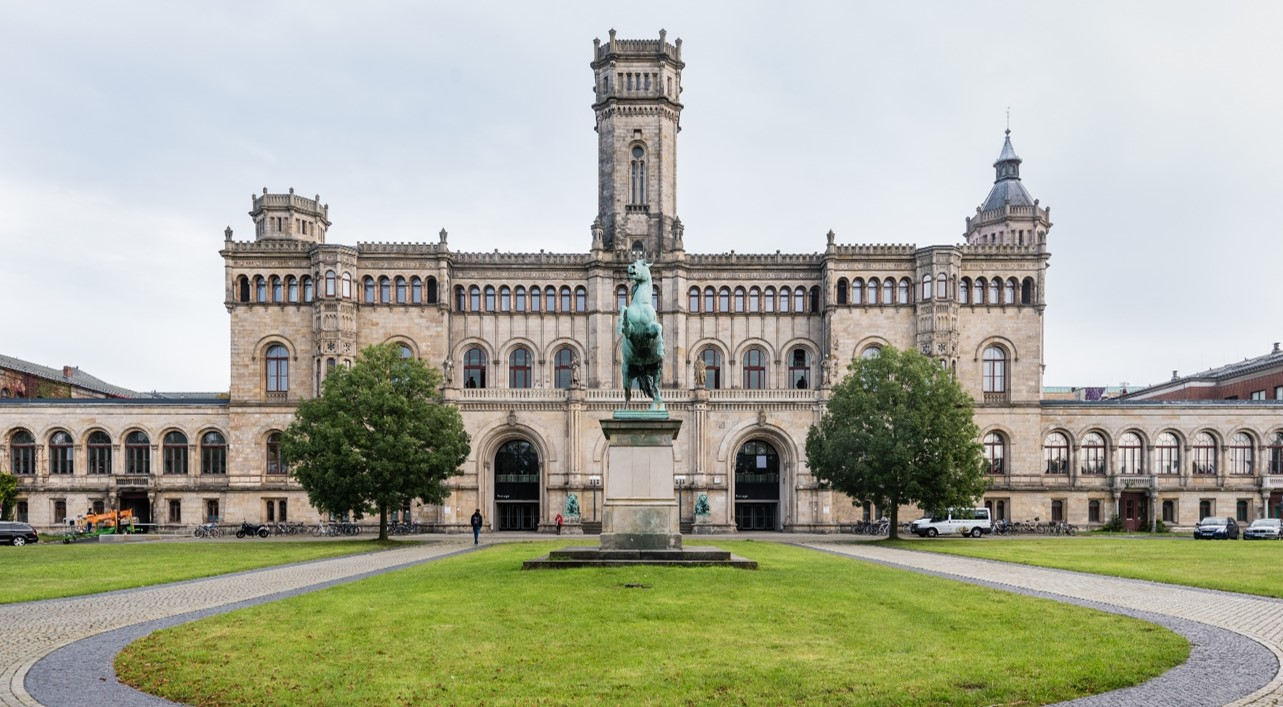
\includegraphics[width=0.75\textwidth]{figures/luh_default_presentation_title_image.jpg}}

\author[Abedjan \& Lindauer]{Ziawasch Abedjan \& Marius Lindauer\\[1em]
	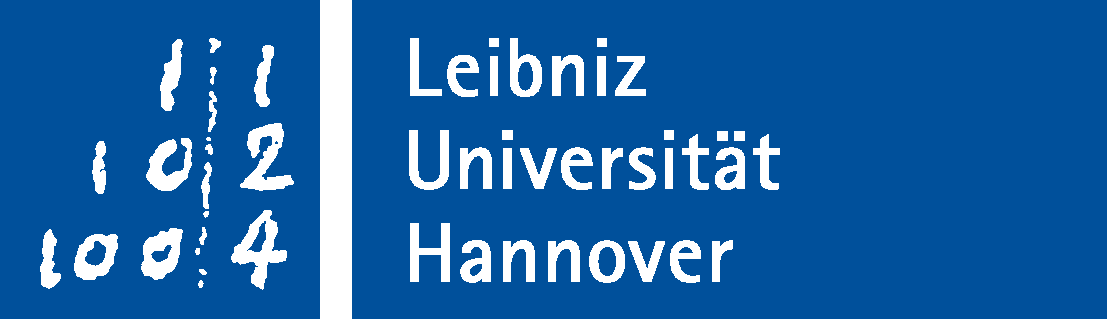
\includegraphics[height=\logoheight]{../latex_main/figures/luh_logo_rgb_0_80_155.pdf}\qquad
	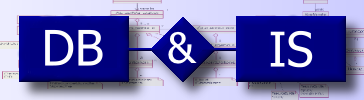
\includegraphics[height=\logoheight]{../latex_main/figures/DBIS_Kurzlogo.png}\qquad

\includegraphics[height=\logoheight]{../latex_main/figures/TNT_darkv4}\qquad

\includegraphics[height=\logoheight]{../latex_main/figures/L3S.jpg}	}
\date{Summer Term 2022; \hspace{0.5em} {
\includegraphics[height=1.5em]{../latex_main/figures/Cc-by-nc-sa_icon.svg.png}}; based on \href{https://ds100.org/fa21/}{[DS100]}
}


%%% Custom Packages
%----------------------------------------------------------------------
% Create dummy content
\usepackage{blindtext}

% Adds a frame with the current page layout. Just call \layout inside of a frame.
\usepackage{layout}


%%% Macros
%\renewcommand{\vec}[1]{\mathbf{#1}}
% \usepackage{bm}
%\let\vecb\bm

\title[Introduction]{DS: Clustering, Part 1}
\subtitle{Agglomerative Clustering}

\graphicspath{ {./figure/} }
%\institute{}


\begin{document}
	
	\maketitle
	\begin{frame}{K-Means}
	    Which clustering result do you like better? 
	    \begin{figure}
	        \centering
	        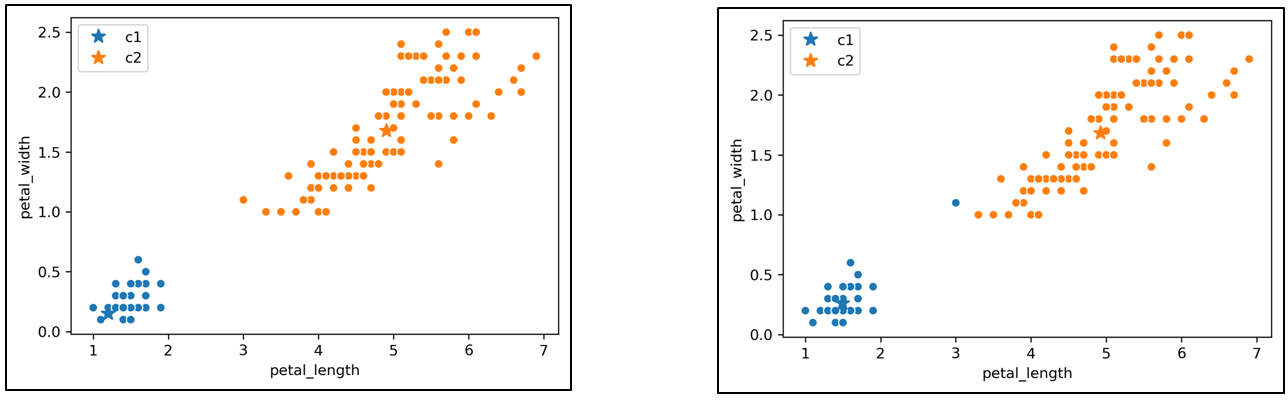
\includegraphics[scale=.4]{Bild27}
	    \end{figure}
	\end{frame}
	
	
	\begin{frame}{K-Means}
	    Which clustering result do you like better? 
	    \begin{figure}
	        \centering
	        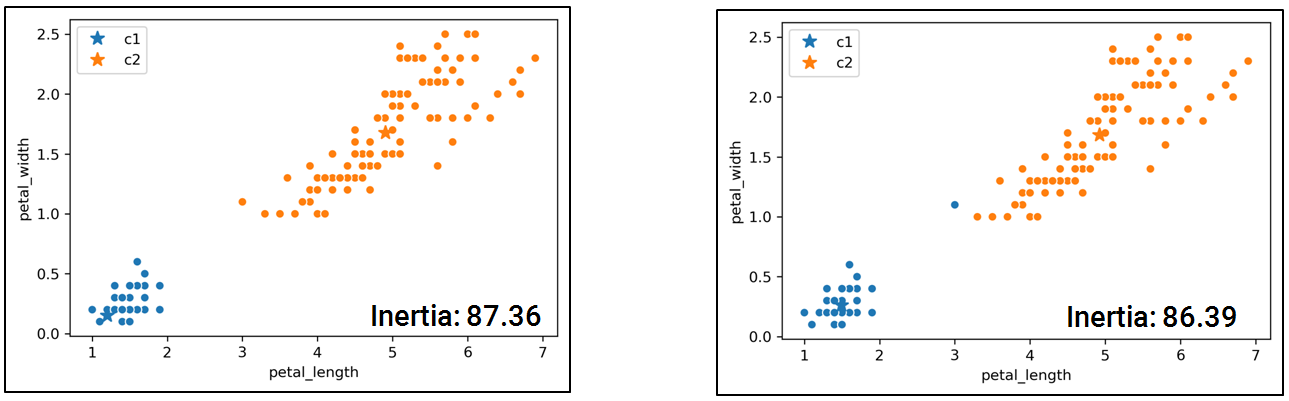
\includegraphics[scale=.35]{Bild28}
	    \end{figure}
	    K-Means likes the one on the right better. It has lower inertia
	    \begin{itemize}
	        \item Why is the inertia on the right lower?
	        \item Is clustering on the right “wrong”?
	    \end{itemize}
	\end{frame}
	
	
	
	\begin{frame}{K-Means}
	    Which clustering result do you like better? 
	    \begin{figure}
	        \centering
	        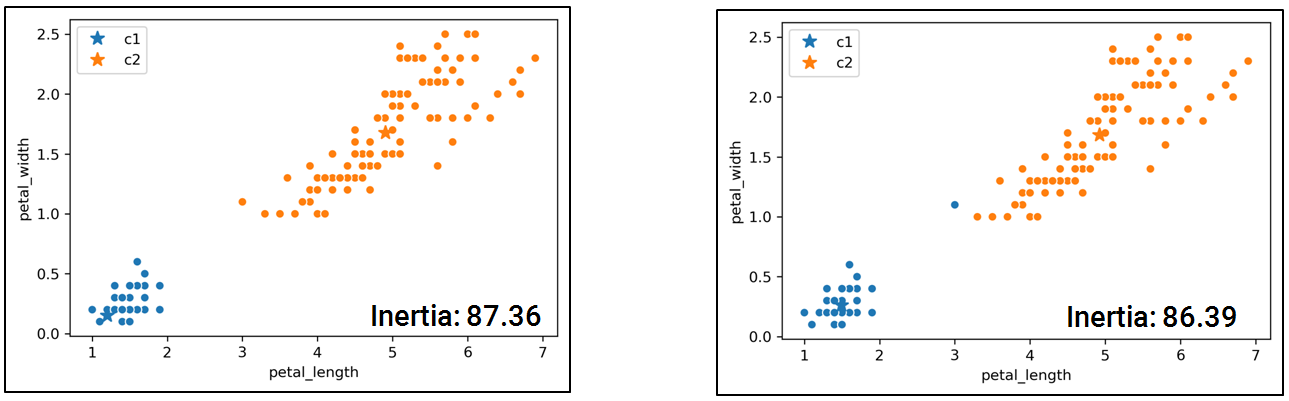
\includegraphics[scale=.35]{Bild28}
	    \end{figure}
	    K-Means likes the one on the right better because it has lower inertia: sum of squared distances from each data point to its center
	    \begin{itemize}
	        \item Why is the inertia lower? K-Means optimizes for distance, not “blobbiness”
	        \item Is clustering on the right “wrong”? Good question! 
	    \end{itemize}
	\end{frame}
	
	
	\begin{frame}{Agglomerative Clustering}
	    As with regression and classification, there are many ways to do clustering\\
	    \bigskip
	    So far we’ve seen K-Means, which attempts to minimize inertia 
	    \begin{itemize}
	        \item Results not guaranteed to optimize inertia
	        \item Even global optimum may not match our intuition of the best result
	    \end{itemize}
	    \bigskip
	    Let’s discuss an alternate idea known as “agglomerative clustering”
	    \begin{itemize}
	        \item Basic idea: 
	        \begin{itemize}
	            \item Every data point starts out as its own cluster
	            \item Join clusters with neighbors until we have only K clusters left
	        \end{itemize}
	    \end{itemize}
	    Let’s see an example for K = 2
	\end{frame}
	
	
	\begin{frame}{Agglomerative Clustering Example}
	    When the algorithm starts, every data point is in its own cluster
	    \begin{itemize}
	        \item Below, 12 data points, so 12 clusters
	        \item Join closest clusters. However, in this case we have a tie: 11 is as close to 1 as it is to 5
	        \item We will break ties arbitrarily
	    \end{itemize}
	    \begin{figure}
	        \centering
	        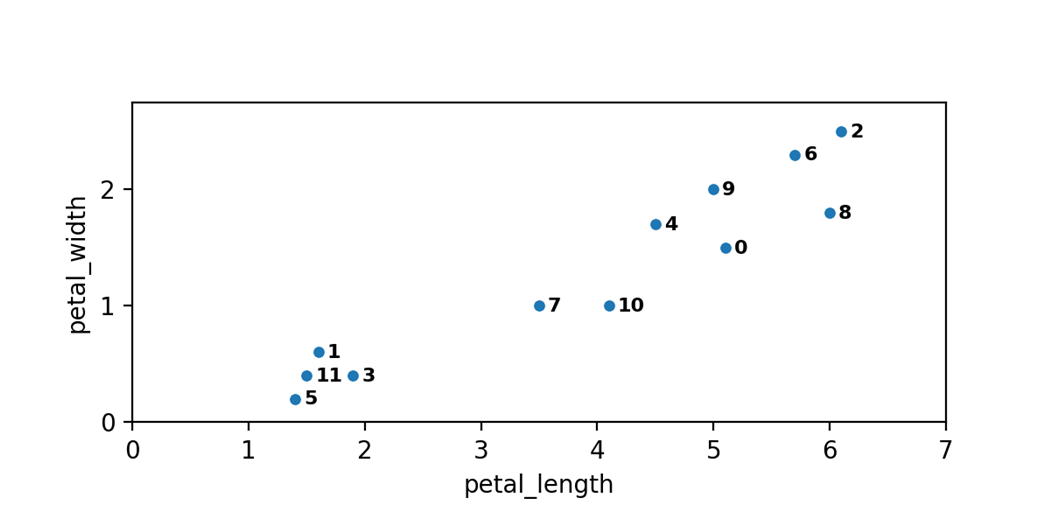
\includegraphics[scale=.5]{Bild29}
	    \end{figure}
	\end{frame}
	
	
	
	\begin{frame}{Agglomerative Clustering Example}
	    When the algorithm starts, every data point is in its own cluster
	    \begin{itemize}
	        \item Below, 12 data points, so 12 clusters
	        \item Merge clusters 1 and 11
	    \end{itemize}
	    \begin{figure}
	        \centering
	        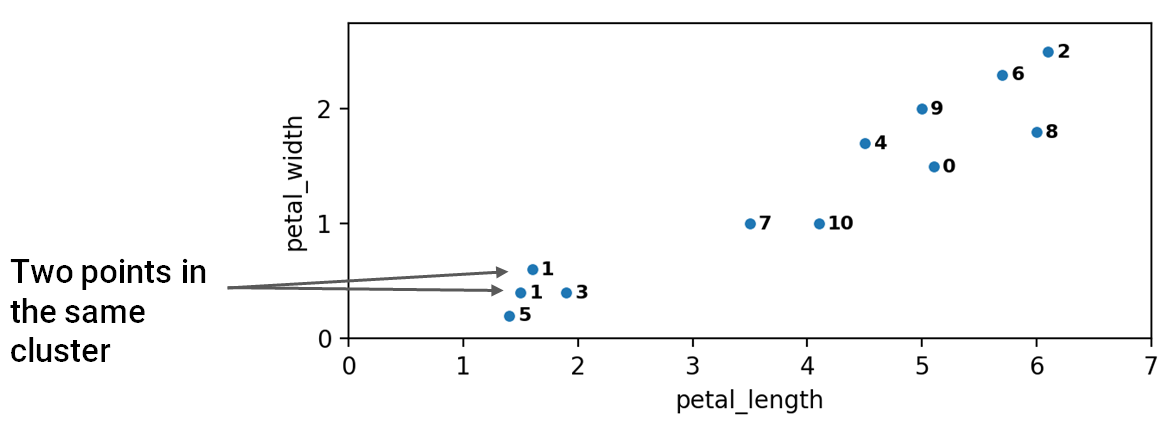
\includegraphics[scale=.35]{Bild30}
	    \end{figure}
	\end{frame}
	
	
	\begin{frame}{Agglomerative Clustering Example}
	    Tricky question:
	    \begin{itemize}
	        \item What is the distance between clusters 1 and 3?
	    \end{itemize}
	    \begin{figure}
	        \centering
	        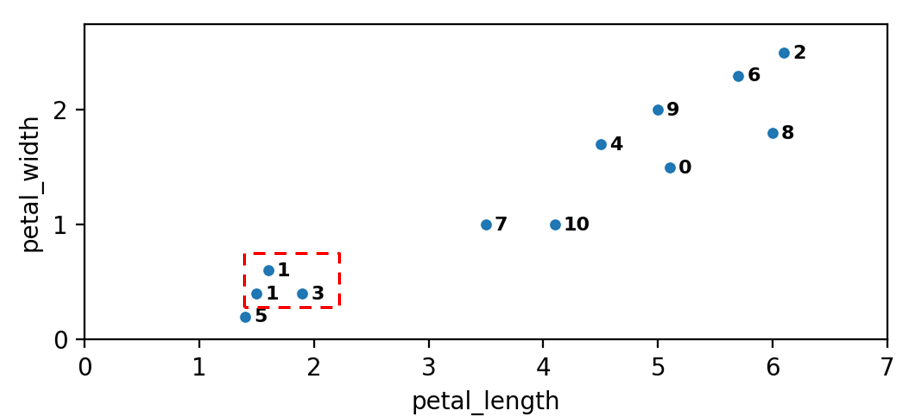
\includegraphics[scale=.35]{Bild31}
	    \end{figure}
	\end{frame}
	
	
	\begin{frame}{Agglomerative Clustering Example}
	    Tricky question:
	    \begin{itemize}
	        \item What is the distance between clusters 1 and 3?
	        \item There is no right answer. Common choice, use the max $\leftarrow$Would be perfectly reasonable to do something else, e.g. average or minimum

	    \end{itemize}
	    \begin{figure}
	        \centering
	        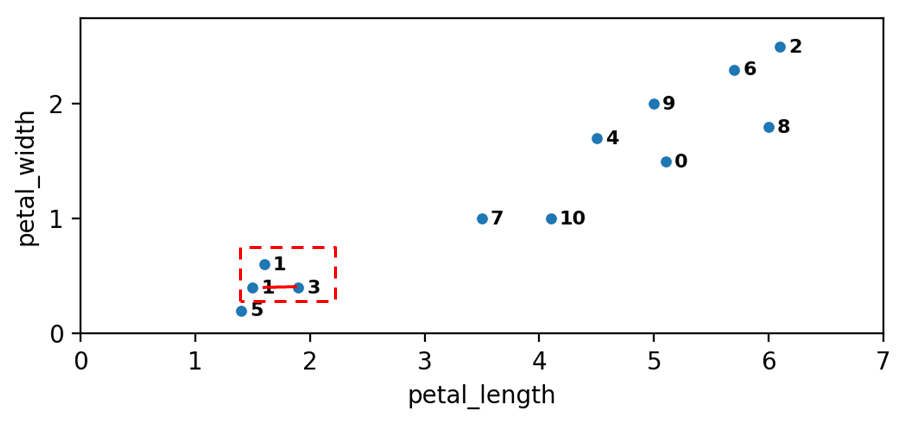
\includegraphics[scale=.35]{Bild32}
	    \end{figure}
	\end{frame}
	
	
	\begin{frame}{Agglomerative Clustering Example}
	    Next two closest are 1 and 3, so merge them
	    \begin{figure}
	        \centering
	        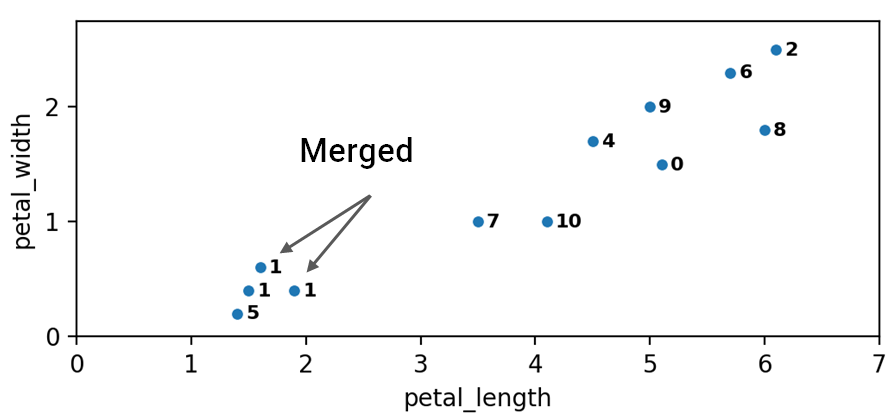
\includegraphics[scale=.35]{Bild33}
	    \end{figure}
	\end{frame}
	
	
	
	\begin{frame}{Agglomerative Clustering Example}
	    Next two closest are 2 and 6, so merge them
	    \begin{figure}
	        \centering
	        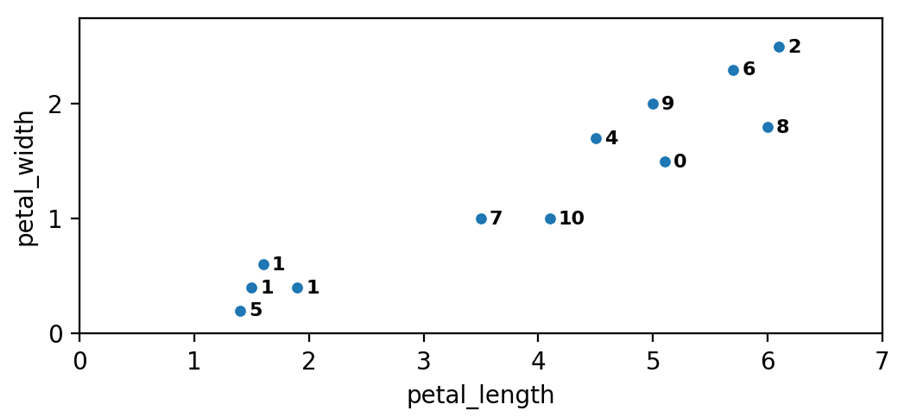
\includegraphics[scale=.35]{Bild34}
	    \end{figure}
	\end{frame}
	
	
	
	\begin{frame}{Agglomerative Clustering Example}
	    Next two closest are 2 and 6, so merge them
	    \begin{figure}
	        \centering
	        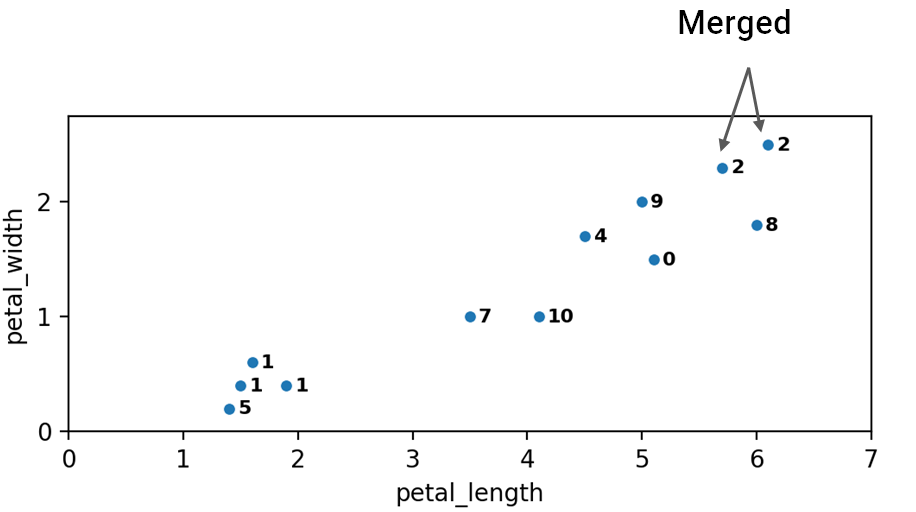
\includegraphics[scale=.35]{Bild35}
	    \end{figure}
	\end{frame}
	
	
	\begin{frame}{Agglomerative Clustering Example}
	    Next two closest are 0 and 9, so merge them
	    \begin{figure}
	        \centering
	        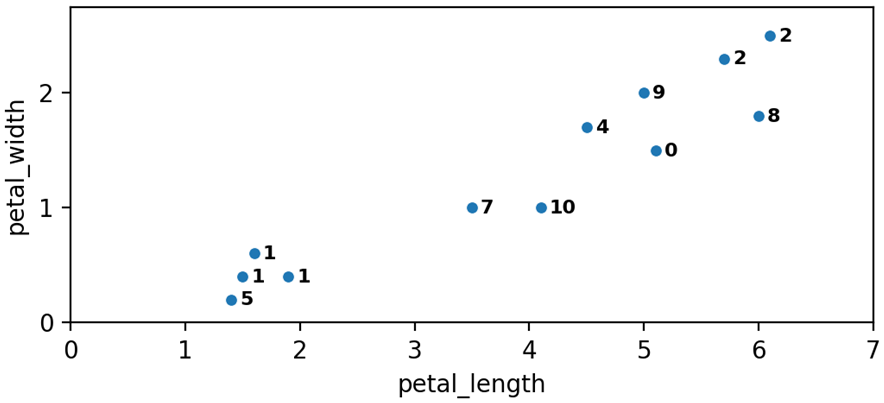
\includegraphics[scale=.35]{Bild36}
	    \end{figure}
	\end{frame}
	
	
	\begin{frame}{Agglomerative Clustering Example}
	    Next two closest are 0 and 9, so merge them
	    \begin{figure}
	        \centering
	        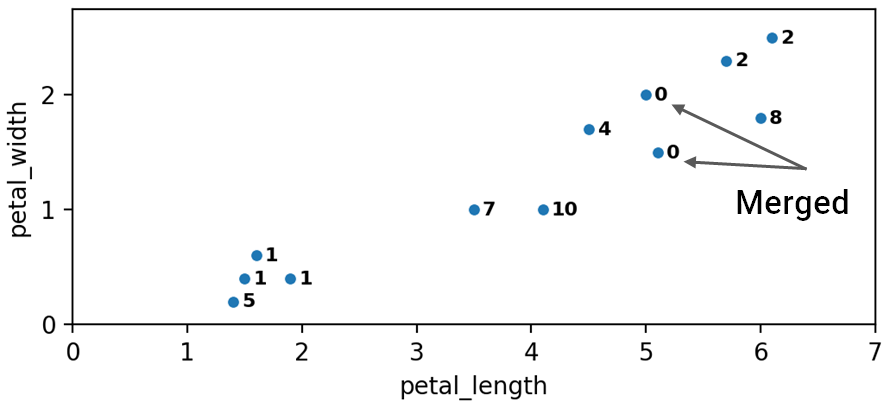
\includegraphics[scale=.35]{Bild37}
	    \end{figure}
	\end{frame}
	
	
	\begin{frame}{Agglomerative Clustering Example}
	    Next two closest are 1 and 5, so merge them
	    \begin{figure}
	        \centering
	        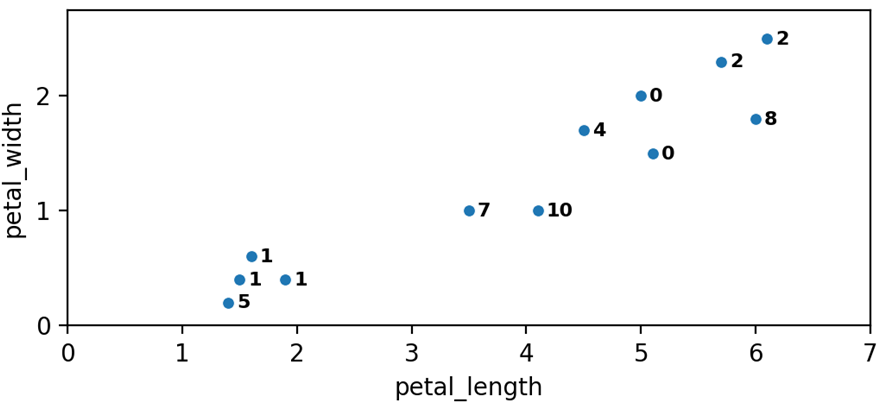
\includegraphics[scale=.35]{Bild38}
	    \end{figure}
	\end{frame}
	
	
	
	\begin{frame}{Agglomerative Clustering Example}
	    Next two closest are 1 and 5, so merge them
	    \begin{figure}
	        \centering
	        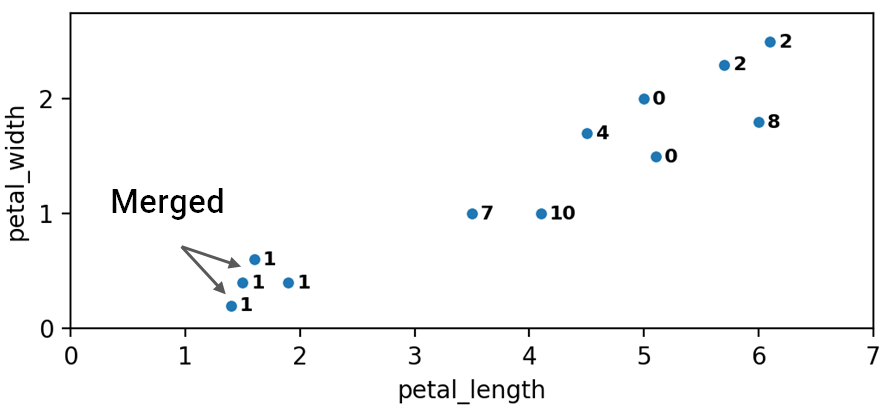
\includegraphics[scale=.35]{Bild39}
	    \end{figure}
	\end{frame}
	
	
	
	\begin{frame}{Agglomerative Clustering Example}
	    Next two closest are 7 and 10, so merge them
	    \begin{figure}
	        \centering
	        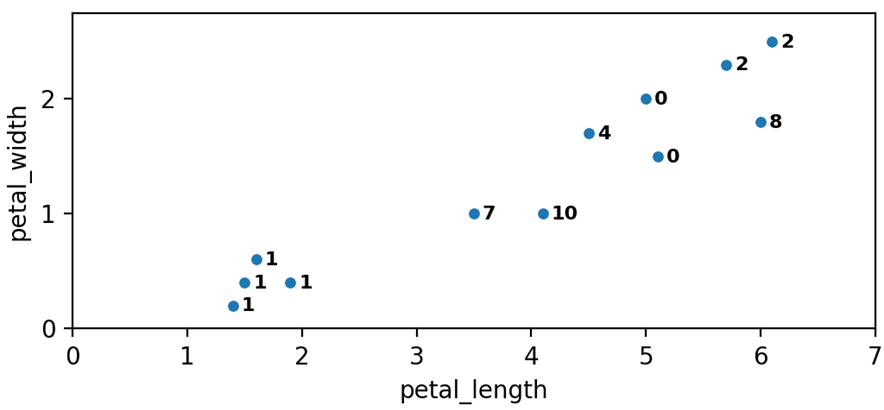
\includegraphics[scale=.35]{Bild40}
	    \end{figure}
	\end{frame}
	
	
	
	\begin{frame}{Agglomerative Clustering Example}
	    Next two closest are 7 and 10, so merge them
	    \begin{figure}
	        \centering
	        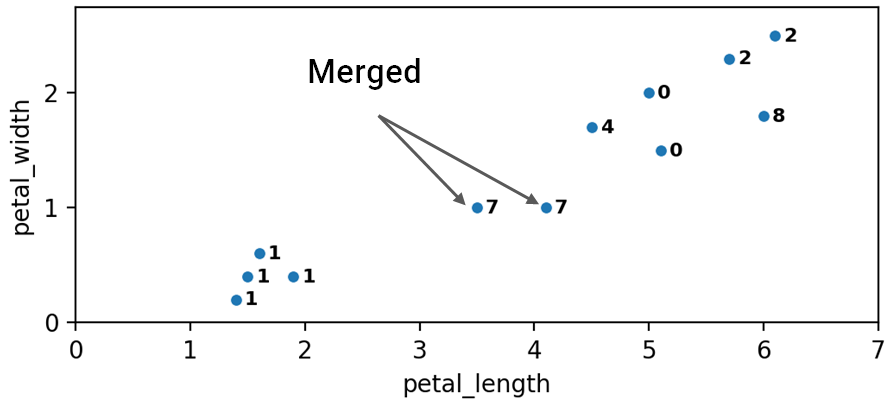
\includegraphics[scale=.35]{Bild41}
	    \end{figure}
	\end{frame}
	
	
	
	\begin{frame}{Agglomerative Clustering Example}
	    Next two closest are 0 and 4, so merge them
	    \begin{figure}
	        \centering
	        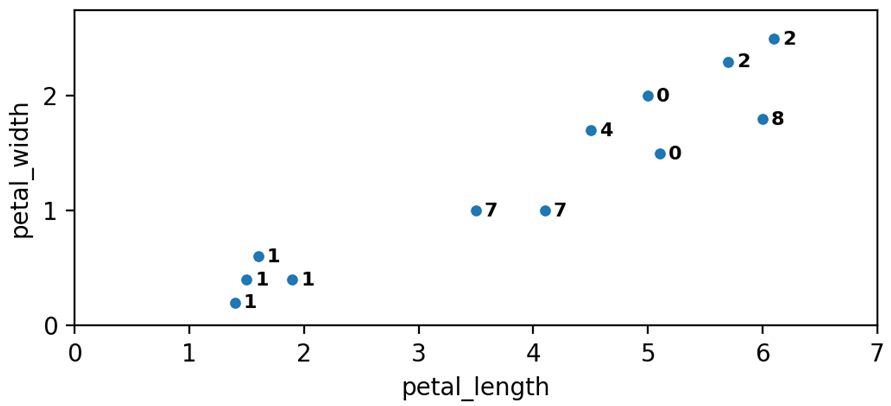
\includegraphics[scale=.35]{Bild42}
	    \end{figure}
	\end{frame}
	
	
	\begin{frame}{Agglomerative Clustering Example}
	    Next two closest are 0 and 4, so merge them
	    \begin{figure}
	        \centering
	        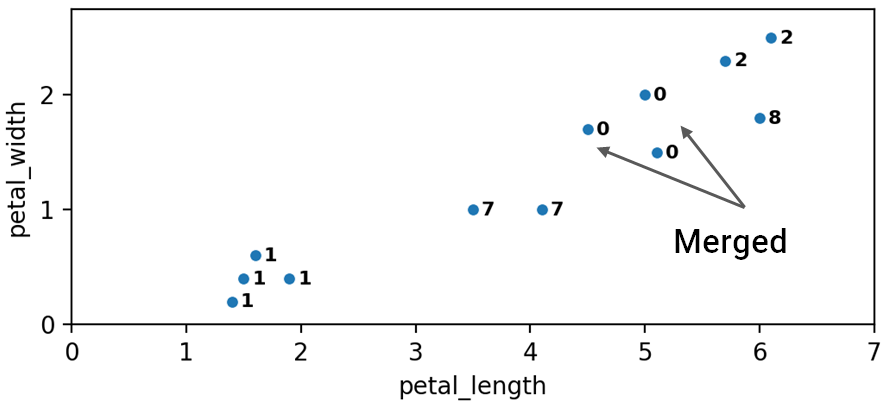
\includegraphics[scale=.35]{Bild43}
	    \end{figure}
	\end{frame}
	
	
	
	\begin{frame}{Agglomerative Clustering Example}
	    We now have 5 clusters:\\
Cluster 0 has 3 points, Cluster 1 has 4 points, Clusters 2 and 7 have 2 points each. Cluster 8 has one point.
	    \begin{figure}
	        \centering
	        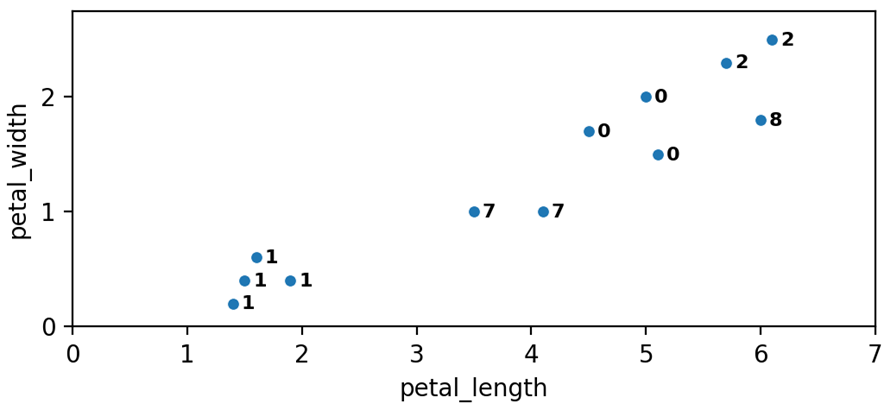
\includegraphics[scale=.35]{Bild44}
	    \end{figure}
	\end{frame}
	
	
	
	\begin{frame}{Agglomerative Clustering Example}
	    Next two closest are 2 and 8, so merge them
	    \begin{figure}
	        \centering
	        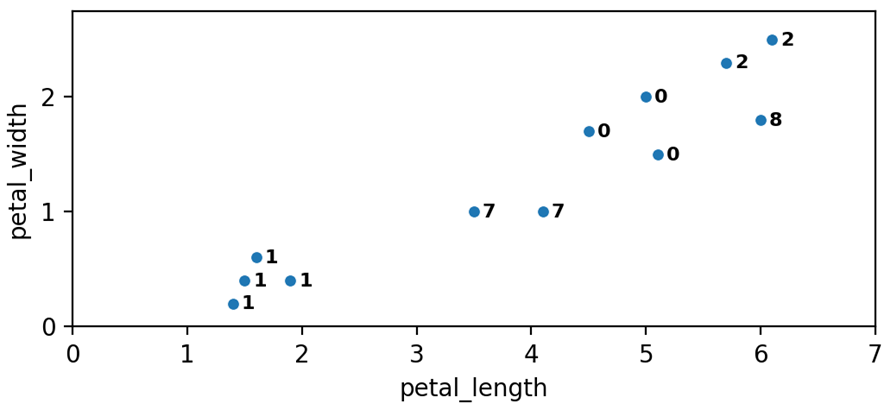
\includegraphics[scale=.35]{Bild44}
	    \end{figure}
	\end{frame}
	
	
	\begin{frame}{Agglomerative Clustering Example}
	    Next two closest are 2 and 8, so merge them
	    \begin{figure}
	        \centering
	        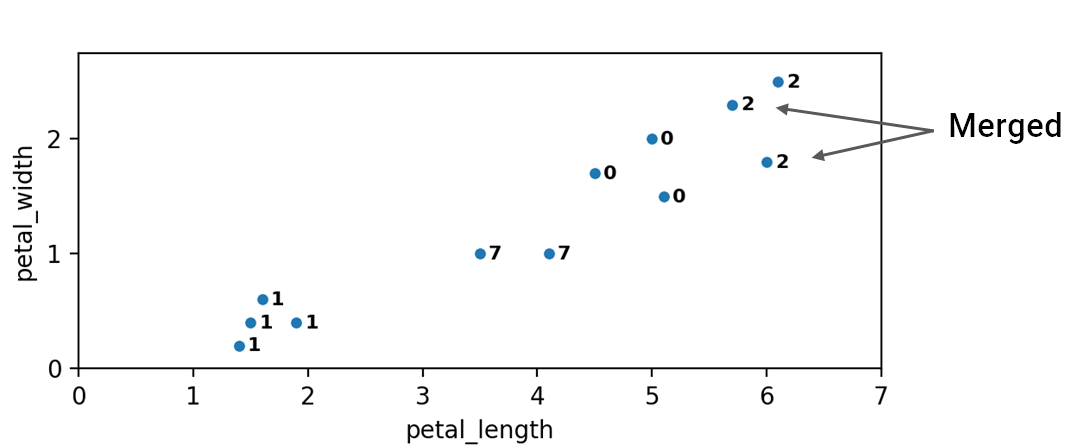
\includegraphics[scale=.35]{Bild45}
	    \end{figure}
	\end{frame}
	
	
	
	\begin{frame}{Agglomerative Clustering Example}
	    Next two closest are 0 and 2, so merge them
	    \begin{figure}
	        \centering
	        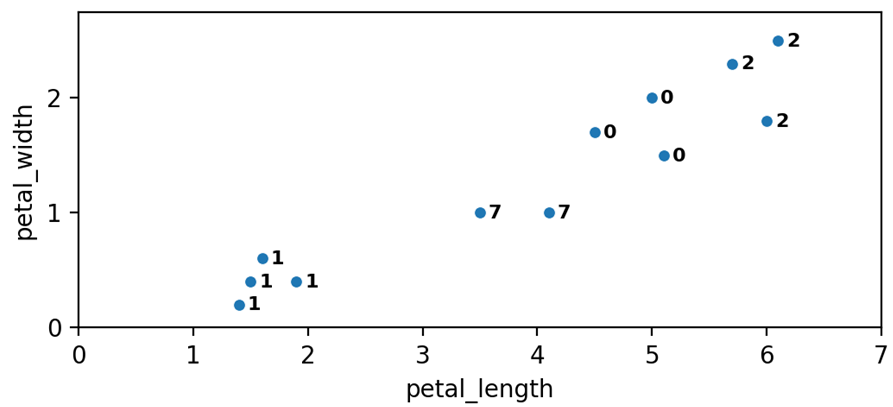
\includegraphics[scale=.35]{Bild46}
	    \end{figure}
	\end{frame}
	
	
	\begin{frame}{Agglomerative Clustering Example}
	    Next two closest are 0 and 2, so merge them
	    \begin{figure}
	        \centering
	        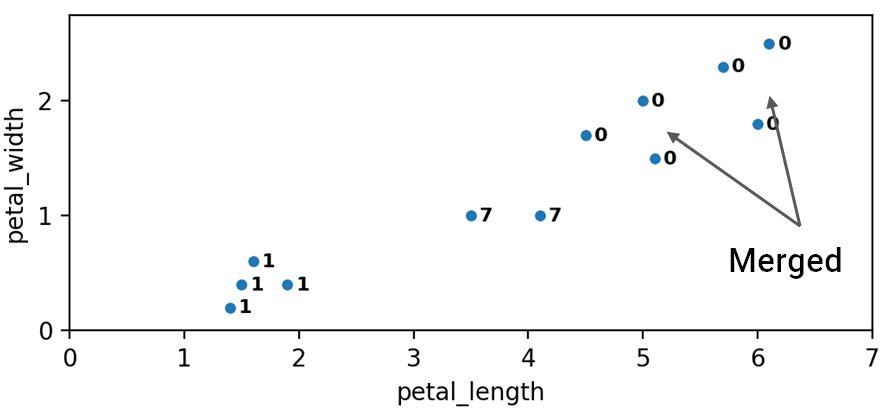
\includegraphics[scale=.35]{Bild47}
	    \end{figure}
	\end{frame}
	
	
	\begin{frame}{Agglomerative Clustering Example}
	    Next up are 1 and 7. Why?
	    \begin{itemize}
	        \item Max line between any member of 1 and 7 is shorter than max line between any member of 0 and 7. Purple line is longer than red line.
	    \end{itemize}
	    \begin{figure}
	        \centering
	        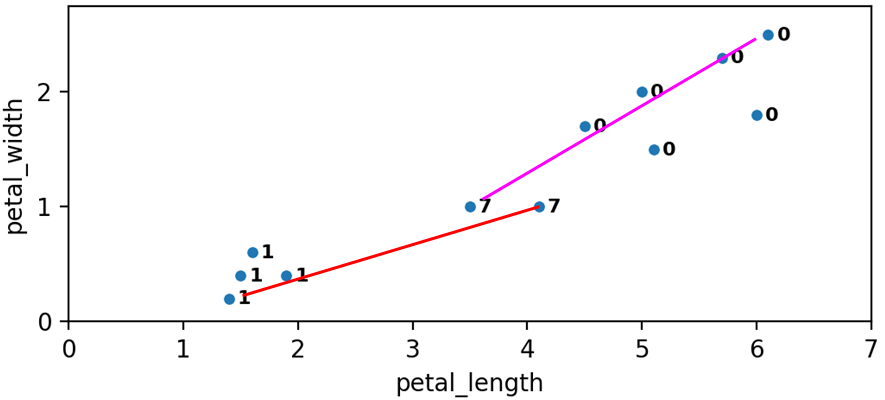
\includegraphics[scale=.35]{Bild48}
	    \end{figure}
	\end{frame}
	
	
	
	\begin{frame}{Agglomerative Clustering Example}
	    Next up are 1 and 7. Why?
	    \begin{itemize}
	        \item Max line between any member of 1 and 7 is shorter than max line between any member of 0 and 7. Purple line is longer than red line.
	    \end{itemize}
	    \begin{figure}
	        \centering
	        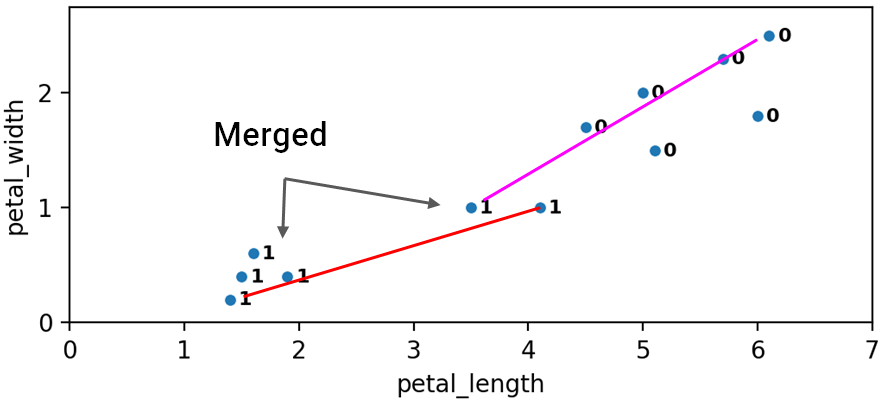
\includegraphics[scale=.35]{Bild49}
	    \end{figure}
	\end{frame}
	
	
	\begin{frame}{Agglomerative Clustering Example}
	    At this point, we are done, because we only have two clusters left.
	    \begin{figure}
	        \centering
	        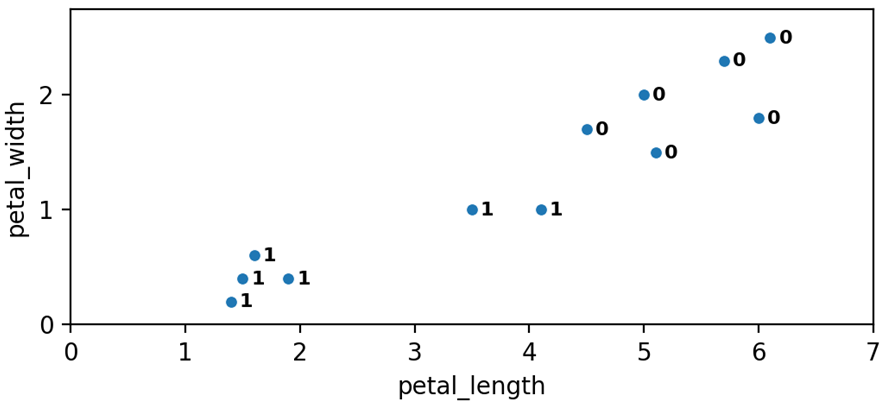
\includegraphics[scale=.35]{Bild50}
	    \end{figure}
	\end{frame}
	
	
	
	\begin{frame}{Agglomerative Clustering Example}
	    On the full dataset, our agglomerative clustering algorithm gets the “right” output
	    \begin{figure}
	        \centering
	        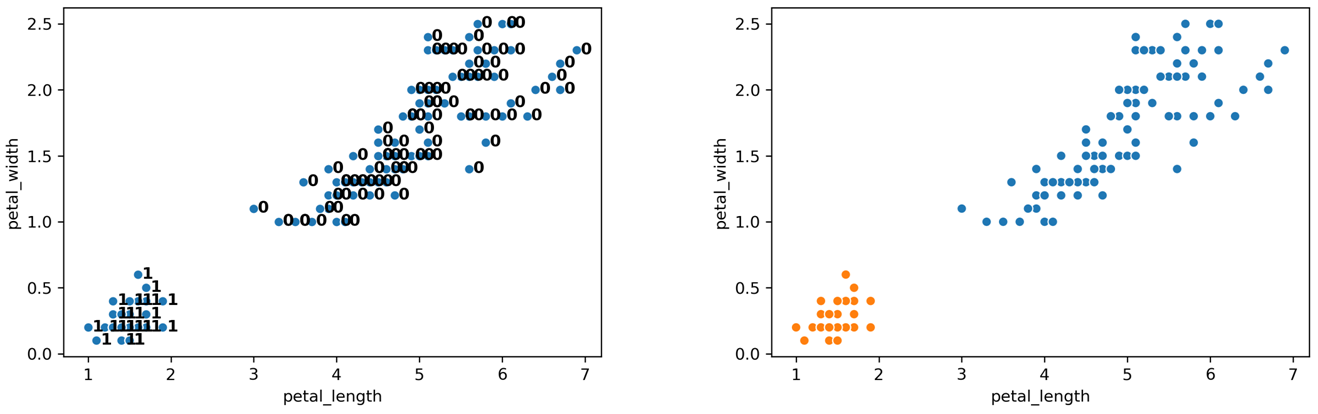
\includegraphics[scale=.35]{Bild51}
	    \end{figure}
	\end{frame}
	
	
	
	\begin{frame}{Clustering and Dendrograms}
	    \begin{columns}
	        \begin{column}{.7\textwidth}
	                Agglomerative clustering is one form of “hierarchical clustering”
	                \begin{itemize}
	                    \item Can keep track of when two clusters got merged 
	                    \begin{itemize}
	                        \item Each cluster is a tree
	                    \end{itemize}
	                    \item Can visualize merging hierarchy, resulting in a “dendrogram”
	                    \begin{itemize}
	                        \item Won’t discuss any further, but you might see these in the wild
	                    \end{itemize}
	                \end{itemize}
	                \begin{figure}
	                    \centering
	                    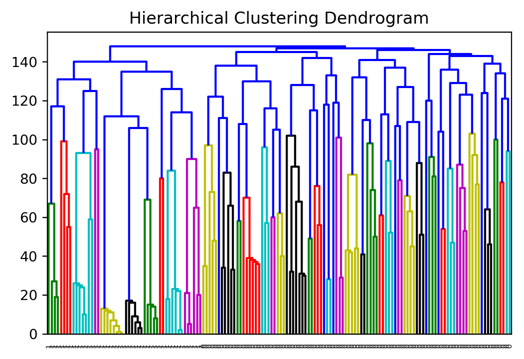
\includegraphics[scale=.6]{Bild52}
	                \end{figure}
	        \end{column}
	        
	        
	        \begin{column}{.3\textwidth}
	                \begin{figure}
	                    \centering
	                    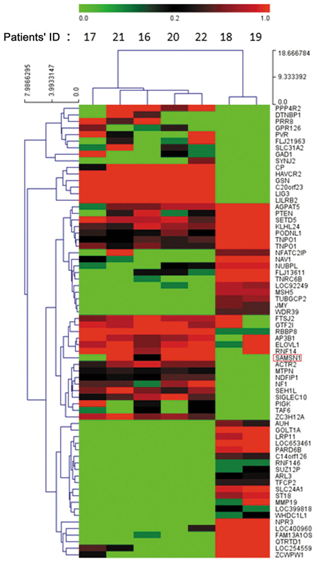
\includegraphics[scale=.6]{Bild53}
	                \end{figure}
	        \end{column}
	    \end{columns}
	\end{frame}
	
	\begin{frame}{Clustering Algorithms: Many More We Haven’t Seen}
	    \begin{figure}
	        \centering
	        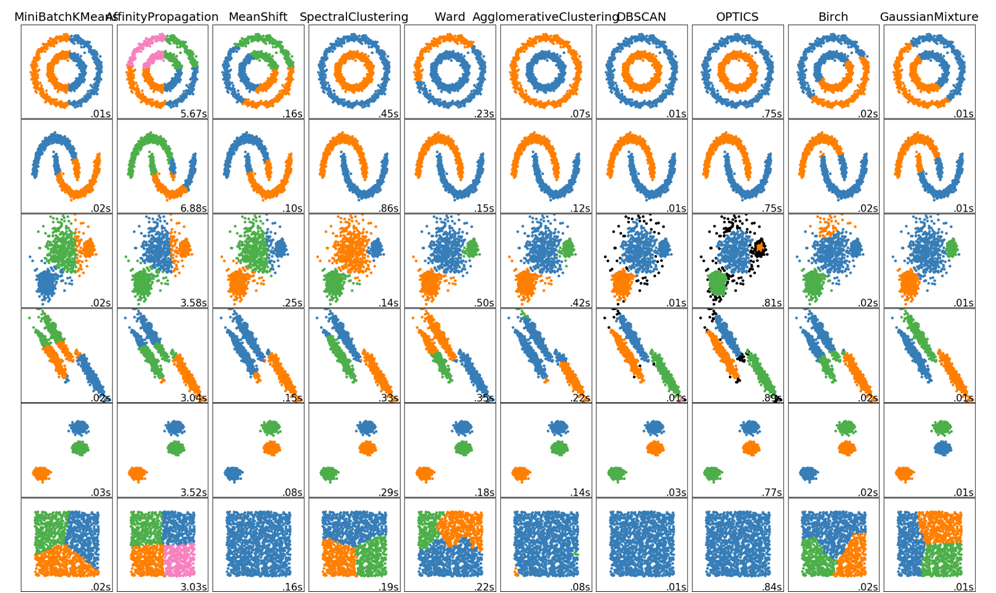
\includegraphics[scale=.5]{Bild54}
	    \end{figure}
	    \url{https://scikit-learn.org/stable/_images/sphx_glr_plot_cluster_comparison_001.png}
	\end{frame}
\end{document}